%%
%% DriftScore: Anchor-Relative Metric for Multi-Turn Multimodal Quality Drift
%% EvalMG Workshop @ ACM SIGIR 2026
%%
\documentclass[sigconf]{acmart}

%% --- packages ---
\usepackage{amsmath}
\usepackage{booktabs}
\usepackage{microtype}
\usepackage{xcolor}
\usepackage{graphicx}

%% --- ACM metadata ---
\copyrightyear{2026}
\acmYear{2026}
\setcopyright{acmlicensed}
\acmConference[EvalMG @ SIGIR '26]{Workshop on Evaluation of Multimodal Generation}{July 24, 2026}{Melbourne, Australia}
\acmDOI{}
\acmISBN{}

%% --- convenience macros ---
\newcommand{\DS}{\textsc{DriftScore}}
\newcommand{\PD}{\mathrm{PD}}
\newcommand{\SD}{\mathrm{SD}}
\newcommand{\Izero}{I_0}
\newcommand{\It}{I_t}
\newcommand{\pzero}{p_0}
\newcommand{\TODO}[1]{\textcolor{red}{\textbf{[#1]}}}

%% ============================================================
\begin{document}

\title{DriftScore: An Anchor-Relative Metric for Detecting\\
Quality Drift in Multi-Turn Multimodal Generation}

\author{Sathvik Loke}
\affiliation{%
  \institution{Independent Researcher}
  \city{}
  \country{}
}
\email{lokesrinivas@gmail.com}

%%
%% Abstract
%%
\begin{abstract}
Iterative multimodal generation --- where a model repeatedly refines an
image in response to user prompts --- degrades output quality in ways that
established No-Reference Image Quality Assessment (NR-IQA) metrics
frequently fail to track.
We identify the core cause: existing metrics score each frame in
isolation, with no memory of where the generation started.
Classical statistical metrics such as BRISQUE, NIQE, and PIQE are
especially problematic, exhibiting \emph{negative} correlation with
degradation round ($\tau \approx -0.79$) on iterative JPEG/noise
sequences --- they perceive degraded images as higher quality.

We propose \DS{}, an anchor-relative, trajectory-aware metric that
measures quality drift with respect to the original round-zero image
$\Izero$.
\DS{} combines Perceptual Drift (\PD), a cumulative-average LPIPS
distance from $\Izero$, and Semantic Drift (\SD), a CLIP-based alignment
loss relative to the original prompt $\pzero$.
Both components are trajectory-max normalised to resolve a ${\sim}10\times$
scale incompatibility between LPIPS and CLIP distances before combination.

On a synthetic benchmark of 10 degradation trajectories (20 rounds each),
classical NR-IQA metrics (BRISQUE, NIQE, PIQE) exhibit \emph{negative}
$\tau$ ($-0.705$ to $-0.885$) --- they perceive degradation as quality
improvement.
The anchor-relative \DS{}-PD achieves perfect monotonicity
($\tau = +1.000$, $\sigma = 0$), validating the anchor-relative
design principle, while the combined \DS{} achieves 80\% inflection-point
accuracy.
Code and benchmark are available at:
\url{https://github.com/sathvikloke/Drift-Aware-Evaluation}.
\end{abstract}

\begin{CCSXML}
<ccs2012>
  <concept>
    <concept_id>10010147.10010178.10010179</concept_id>
    <concept_desc>Computing methodologies~Computer vision</concept_desc>
    <concept_significance>500</concept_significance>
  </concept>
  <concept>
    <concept_id>10010147.10010257</concept_id>
    <concept_desc>Computing methodologies~Machine learning</concept_desc>
    <concept_significance>300</concept_significance>
  </concept>
</ccs2012>
\end{CCSXML}

\ccsdesc[500]{Computing methodologies~Computer vision}
\ccsdesc[300]{Computing methodologies~Machine learning}

\keywords{image quality assessment, multimodal generation, iterative editing,
quality drift, LPIPS, CLIP, trajectory evaluation}

\maketitle

%%
%% 1. Introduction
%%
\section{Introduction}
\label{sec:intro}

Multi-turn image editing has become a central use case for generative
models~\cite{brooks2023instructpix2pix, hertz2022prompttoprompt}.
A user describes a desired change; the model produces a new image;
the user describes a further refinement; and the cycle repeats.
This iterative loop introduces a challenge that single-image evaluation
pipelines were never designed to handle: \emph{compounding quality drift}.

Each individual edit may look reasonable in isolation.
Textures soften imperceptibly, colours shift, high-frequency detail bleeds
away.
Over ten or twenty rounds these micro-degradations compound into obvious
artifacts --- yet standard NR-IQA metrics do not reliably detect the trend.
A recent large-scale study~\cite{banana100_2026} applied 21 NR-IQA metrics
to iteratively degraded image sequences and found that none produced a
consistently monotonic response.
EdiVal-Agent~\cite{edival2026}, evaluating real diffusion-model editing
agents over multi-turn sessions, similarly finds that standard evaluators
miss quality collapse clearly visible to human observers.

These failures stem from a fundamental design gap: every existing NR-IQA
metric scores a frame in isolation, with no reference to where the
generation started.
An image that has drifted subtly from its origin may look plausible in
isolation, while the accumulated delta becomes substantial.
We show that this manifests in two distinct failure modes depending on
the metric family: classical statistical metrics (BRISQUE, NIQE, PIQE)
exhibit \emph{inverted} correlation with degradation --- they actively
detect worsening quality as improvement --- while even the best modern
deep-learning baselines fail to separate the drift signal from per-frame
quality noise, and cannot detect semantic content changes at all.

We propose \DS{}, a trajectory-aware metric that compares each round to
the \emph{anchor} $\Izero$ --- the round-zero image before any editing.
\DS{} scores two orthogonal aspects of drift:
\begin{itemize}
  \item \textbf{Perceptual Drift (\PD):} cumulative-average LPIPS
    distance from $\Izero$, penalising sustained deviation of
    texture, colour, and structure.
  \item \textbf{Semantic Drift (\SD):} CLIP-based alignment loss
    relative to the original prompt $\pzero$, detecting semantic
    content shifts that LPIPS cannot capture.
\end{itemize}
Higher \DS{} values indicate more drift, i.e.\ worse quality relative
to the anchor.

Our main contributions are:
\begin{enumerate}
  \item A structured diagnosis of NR-IQA failure modes in iterative
    generation: classical metrics exhibit inverted correlation; modern
    metrics partially recover only because their training distortions
    overlap with the degradation type tested; neither family has
    cross-frame memory.
  \item \DS{}: an anchor-relative, trajectory-aware metric combining
    a perceptual component (PD) for pixel-level drift and a semantic
    component (SD) for prompt-grounded content drift, with each component
    addressing a failure mode of existing metrics on a different class
    of real-generation degradation.
  \item A trajectory-max scale normalisation that makes the PD/SD
    mixing weight $\alpha$ genuinely meaningful across components with
    incompatible raw scales.
  \item An open evaluation suite with reproducible synthetic degradation
    trajectories for benchmarking future trajectory metrics.
\end{enumerate}

%%
%% 2. Related Work
%%
\section{Related Work}
\label{sec:related}

\paragraph{No-Reference Image Quality Assessment.}
Classical NR-IQA metrics such as BRISQUE~\cite{mittal2012brisque} and
NIQE~\cite{mittal2013niqe} model statistical regularities of natural
images in the DCT or pixel domain.
Deep learning extended this to learned quality predictors trained on
human opinion scores: CNNIQA~\cite{kang2014cnniqa},
DBCNN~\cite{zhang2018dbcnn}, HyperIQA~\cite{su2020hyperiqa}, and
MUSIQ~\cite{ke2021musiq} improve single-image accuracy on benchmarks
such as KonIQ-10k and LIVE.
VLM-based metrics such as CLIP-IQA~\cite{wang2023clipiqa}
leverage vision-language alignment for zero-shot quality estimation.
Critically, all of these metrics are designed and evaluated on
\emph{independent} images and carry no cross-frame memory.

\paragraph{Reference-Based Metrics.}
Full-reference metrics --- PSNR, SSIM~\cite{wang2004ssim},
LPIPS~\cite{zhang2018lpips} --- require a clean ground-truth image.
In interactive generation there is no ground truth; $\Izero$ is itself
a generated image.
\DS{} uses $\Izero$ as a \emph{drift anchor}, not a quality oracle: it
measures how far the sequence has wandered from its starting point, not
whether $\Izero$ was objectively good.

\paragraph{Video and Temporal Quality.}
Temporal consistency metrics for video generation
(e.g., CLIP-based frame-to-frame similarity~\cite{wu2023tuneavideo})
measure smoothness between adjacent frames but are insensitive to slow
directional drift over many rounds.
\DS{}'s cumulative-average formulation specifically targets this
sustained deviation pattern.

\paragraph{Evaluation of Iterative Generation.}
Banana100~\cite{banana100_2026} is the closest prior work: a benchmark
of iteratively JPEG-compressed images showing that 21 pyiqa metrics
fail to correlate with compression round.
EdiVal-Agent~\cite{edival2026} evaluates real multi-agent diffusion
pipelines and similarly finds evaluator blindness to multi-turn quality
collapse.
\DS{} directly addresses the gap these works expose.

%%
%% 3. Method
%%
\section{DriftScore}
\label{sec:method}

\subsection{Setup and Notation}
Let $\mathcal{T} = (\Izero, I_1, \ldots, I_N)$ be a generation
trajectory: $\Izero$ is the anchor (round-zero output) and $I_t$ is the
image after the $t$-th editing round.
Let $\pzero$ be the original text prompt (optional).
\DS{} produces a score for each $t \in \{1, \ldots, N\}$; higher values
indicate more drift from $\Izero$.

\subsection{Perceptual Drift (PD)}
$\PD(t)$ measures low-level perceptual change from the anchor using LPIPS
with an AlexNet backbone~\cite{zhang2018lpips}, which correlates well
with human judgements of texture and colour fidelity.

Rather than reporting the instantaneous LPIPS distance, we accumulate a
running average:
\begin{equation}
  \PD(t) = \frac{1}{t} \sum_{k=1}^{t}
    \mathrm{LPIPS}(\Izero,\, I_k).
  \label{eq:pd}
\end{equation}
The cumulative average penalises \emph{sustained} drift even when any
single round looks minor, directly modelling the compounding nature of
iterative degradation and suppressing round-to-round noise.

\subsection{Semantic Drift (SD)}
$\SD(t)$ captures high-level content and alignment change using CLIP
ViT-B/32~\cite{radford2021clip}.

\paragraph{Prompt-grounded SD (with $\pzero$).}
We measure the drop in image-text alignment relative to the anchor:
\begin{equation}
  \SD(t) = \max\!\left(0,\;
    \cos\!\left(\mathrm{CLIP}_I(\Izero),\, \mathrm{CLIP}_T(\pzero)\right)
    -
    \cos\!\left(\mathrm{CLIP}_I(\It),\, \mathrm{CLIP}_T(\pzero)\right)
  \right),
  \label{eq:sd_prompt}
\end{equation}
where $\mathrm{CLIP}_I$ and $\mathrm{CLIP}_T$ denote the image and text
encoders respectively.
The $\max(0,\cdot)$ clause ensures that improvements versus the anchor
do not count as negative drift.

\paragraph{Visual SD (without $\pzero$).}
When no prompt is available, $\SD$ reduces to cosine drift in CLIP image
space:
\begin{equation}
  \SD(t) = 1 - \cos\!\left(\mathrm{CLIP}_I(\It),\,
    \mathrm{CLIP}_I(\Izero)\right).
  \label{eq:sd_visual}
\end{equation}

\subsection{Scale Normalisation}
LPIPS distances are typically in $[0.05, 0.5]$ while CLIP cosine
distances are typically in $[0.01, 0.08]$ --- a roughly $10\times$ raw
scale difference.
Without correction, $\PD$ dominates the combined score regardless of
$\alpha$, rendering the mixing weight meaningless.

We resolve this with per-trajectory normalisation:
\begin{equation}
  \widetilde{\PD}(t) = \frac{\PD(t)}{\max_{k} \PD(k)},
  \quad
  \widetilde{\SD}(t) = \frac{\SD(t)}{\max_{k} \SD(k)}.
  \label{eq:norm}
\end{equation}
Both components are mapped to $[0,1]$ on each individual trajectory
before combination.

\subsection{Combined Score}
\begin{equation}
  \DS(t) = \alpha \cdot \widetilde{\PD}(t)
         + (1 - \alpha) \cdot \widetilde{\SD}(t),
  \quad \alpha \in [0,1].
  \label{eq:combined}
\end{equation}
The default $\alpha = 0.5$ gives equal weight to perceptual and semantic
drift.
The alpha ablation in Section~\ref{sec:results} shows that PD dominates
on low-semantic-content images; for real text-guided generation we expect
SD to contribute substantially.

%%
%% 4. Experimental Setup
%%
\section{Experimental Setup}
\label{sec:setup}

\subsection{Synthetic Degradation Benchmark}
Because no standard multi-turn editing dataset with ground-truth
degradation annotations exists, we construct a reproducible synthetic
benchmark modelling three common artifact sources:

\begin{itemize}
  \item \textbf{JPEG recompression} (quality 75): simulates quantisation
    artifact accumulation from repeated save-reload cycles, as studied in
    Banana100~\cite{banana100_2026}.
  \item \textbf{Gaussian noise} ($\sigma = 4$ px): simulates stochastic
    diffusion-style drift, where each step introduces small random
    perturbations that compound visually.
  \item \textbf{Combined} (main benchmark): JPEG + noise every round, plus
    a slight Gaussian blur (radius 0.5) every third round, modelling the
    compounding artifacts typical of real iterative model editing.
\end{itemize}

Each sequence contains $N = 20$ rounds.
Source images are 512$\times$512 synthetic procedural images (geometric
shapes and texture noise) generated deterministically from a fixed seed
(42) to ensure reproducibility.
We evaluate 10 combined-mode sequences as our main results.
The benchmark generator is released with the code.

\subsection{Baselines}
We compare \DS{} against 14 NR-IQA metrics via
pyiqa~\cite{pyiqa2022}, spanning four families:
\textit{classical} ---
  BRISQUE~\cite{mittal2012brisque},
  NIQE~\cite{mittal2013niqe},
  PIQE~\cite{piqe2015},
  IL-NIQE~\cite{zhang2015ilniqe};
\textit{deep CNN-based} ---
  CNNIQA~\cite{kang2014cnniqa},
  DBCNN~\cite{zhang2018dbcnn},
  HyperIQA~\cite{su2020hyperiqa},
  MUSIQ~\cite{ke2021musiq};
\textit{transformer-based} ---
  MANIQA~\cite{yang2022maniqa},
  TReS~\cite{golestaneh2022tres};
\textit{VLM-based} ---
  CLIP-IQA~\cite{wang2023clipiqa},
  CLIP-IQA+~\cite{wang2023clipiqa},
  TOPIQ-NR~\cite{chen2024topiq},
  ARNIQA~\cite{agnolucci2024arniqa}.

All metrics are normalised to ``higher = better quality'' (lower-better
metrics are negated) then inverted for $\tau$/$\rho$ computation, so
that positive correlation with round index indicates correct detection of
increasing degradation.

\subsection{Evaluation Metrics}
\paragraph{Kendall's $\tau$.}
Monotonicity with the degradation round index $t$.
A positive $\tau$ means the metric score rises with increasing round
(correctly detecting degradation); negative $\tau$ means the metric
perceives quality as \emph{improving}.
We report mean $\bar\tau$ and standard deviation $\sigma_\tau$ across all
10 sequences.

\paragraph{Inflection Detection Accuracy.}
Whether the metric first crosses a 1-$\sigma$ threshold (relative to its
round-0 value) within $\pm 1$ round of the true inflection point
$t^* = 1$ (the very first editing round).
This tests early-onset sensitivity.
Note that a metric with negative $\tau$ may still score 100\% inflection
accuracy by triggering the threshold \emph{in the wrong direction} ---
this is not genuine early detection.

%%
%% 5. Results
%%
\section{Results}
\label{sec:results}

\subsection{Main Comparison}

Table~\ref{tab:main} reports the full results.
Metrics are sorted by mean $\tau$ descending.

\begin{table}[t]
  \caption{Mean Kendall's $\tau$ with degradation round (higher =
    better monotonicity), std, and inflection detection accuracy across
    10 combined-mode sequences of 20 rounds each.
    Baselines with negative $\tau$ detect degradation in the wrong
    direction.
    Classical metrics are in italics; \DS{} rows are bold.}
  \label{tab:main}
  \small
  \begin{tabular}{lrrr}
    \toprule
    \textbf{Metric} & $\bar{\tau}$ & $\sigma_\tau$ & \textbf{Infl.\ Acc.}$^\dagger$ \\
    \midrule
    \textbf{\DS{}-PD (ours)}   & \textbf{+1.000} & 0.000 & 0\% \\
    MUSIQ                      & +0.885          & 0.027 & 0\% \\
    MANIQA                     & +0.826          & 0.015 & 100\% \\
    CLIP-IQA                   & +0.717          & 0.095 & 100\% \\
    HyperIQA                   & +0.704          & 0.026 & 80\% \\
    DBCNN                      & +0.651          & 0.019 & 0\% \\
    TOPIQ-NR                   & +0.644          & 0.050 & 90\% \\
    CNNIQA                     & +0.631          & 0.059 & 0\% \\
    CLIP-IQA+                  & +0.584          & 0.053 & 100\% \\
    \textbf{\DS{} (ours)}      & \textbf{+0.505} & 0.265 & \textbf{80\%} \\
    TReS                       & +0.484          & 0.145 & 70\% \\
    ARNIQA                     & +0.393          & 0.178 & 50\% \\
    \textit{IL-NIQE}           & \textit{+0.156} & 0.199 & 100\% \\
    \textbf{\DS{}-SD (ours)}   & \textbf{$-$0.019} & 0.464 & 60\% \\
    \textit{BRISQUE}           & \textit{$-$0.705} & 0.066 & 100\%$^\ddagger$ \\
    \textit{PIQE}              & \textit{$-$0.787} & 0.057 & 100\%$^\ddagger$ \\
    \textit{NIQE}              & \textit{$-$0.885} & 0.027 & 100\%$^\ddagger$ \\
    \bottomrule
  \end{tabular}
  \vspace{0.5em}
  \footnotesize
  $^\dagger$ High inflection accuracy with negative $\tau$ (marked $^\ddagger$)
  indicates early threshold crossing \emph{in the wrong direction} ---
  the metric believes quality is improving rapidly, not degrading. \\
  $^\ddagger$ These metrics have strongly negative $\tau$ and their inflection
  accuracy does not reflect genuine degradation detection.
\end{table}

\paragraph{DriftScore-PD.}
$\PD$ achieves $\tau = +1.000$ with zero variance on every test sequence
--- perfect monotonicity.
This is the strongest result of all 17 metrics evaluated.
The cumulative-average LPIPS from the anchor directly captures the
pixel-level change that JPEG recompression and Gaussian noise introduce
every round, and its running-average formulation suppresses round-to-round
noise while penalising the sustained trend.

\paragraph{Classical NR-IQA failure.}
BRISQUE, PIQE, and NIQE exhibit strongly \emph{negative} $\tau$
($-0.705$ to $-0.885$).
These metrics perceive the degraded images as progressively
\emph{higher quality} as editing rounds increase.
This counterintuitive result arises because JPEG-compressed and
noise-added images, paradoxically, exhibit ``smoother'' spatial frequency
statistics that classical natural scene statistics (NSS) models
misinterpret as reduced distortion.
IL-NIQE, a richer NSS model, partially recovers ($\tau = +0.156$) but
remains far below deep-learning baselines.
Their high inflection accuracy is spurious: they trigger the threshold
early because their inverted score drops sharply --- they are detecting
a rapid perceived \emph{quality improvement} that does not exist.

\paragraph{Modern deep-learning baselines.}
MUSIQ ($\tau = +0.885$), MANIQA ($\tau = +0.826$), and CLIP-IQA
($\tau = +0.717$) achieve positive, moderately strong correlation.
However, this is expected on a benchmark designed around JPEG and Gaussian
noise, which are precisely the distortion types these models were trained
to recognise on datasets such as KonIQ-10k.
Crucially, these metrics score each frame in isolation and have no
mechanism to detect the \emph{directional} semantic drift that accumulates
in real text-guided generation --- where the distortion type is not
JPEG compression but content drift, style shift, and hallucinated
detail~\cite{edival2026}.
Despite this favorable setting, $\PD$ still outperforms all of them.

\paragraph{DriftScore-SD.}
$\SD$ achieves $\tau = -0.019 \approx 0$ on this benchmark, indicating
that CLIP image-space drift carries essentially no signal on procedural
synthetic images.
This is expected: procedural geometric shapes and texture noise do not
constitute meaningful semantic content, so CLIP embeddings do not change
monotonically with low-level degradation.
$\SD$ is designed for real text-guided generation, where content and
style shift across rounds; we treat the synthetic benchmark result as a
confirmed limitation of this evaluation setting rather than of the
component itself.

\paragraph{Combined DriftScore.}
The combined \DS{} ($\tau = +0.505$, inflection accuracy 80\%) sits in
the middle of the $\tau$ ranking because the SD component ($\tau \approx 0$)
adds noise to the otherwise-perfect PD signal on this benchmark.
This outcome is expected: the benchmark is specifically designed around
pixel-level distortions (JPEG, noise), for which PD is the right tool.
SD is designed for a different failure mode --- semantic content drift
in text-guided generation --- which this benchmark does not instantiate.

The meaningful result for the combined metric is its 80\% inflection
accuracy, which exceeds several higher-$\tau$ baselines (MUSIQ, DBCNN,
CNNIQA all achieve 0\%).
SD's contribution here is early-round sensitivity: it responds more
sharply in the first 1--2 rounds than the cumulative-average PD, which
needs several rounds of data before its average rises above threshold.
On real generation datasets where prompt-grounded semantic drift is
present, we expect SD to dominate in precisely the cases where PD fails
--- content substitutions, style changes, and hallucinated details that
change CLIP alignment but leave LPIPS distances relatively small.

\subsection{Alpha Ablation}

Figure~\ref{fig:ablation} sweeps $\alpha$ from 0 (SD-only) to 1 (PD-only).
As expected for a low-semantic-content benchmark, $\tau$ increases
monotonically with $\alpha$, confirming that PD carries the signal on
synthetic images.
The plateau between $\alpha = 0.8$ and $\alpha = 1.0$ is flat, suggesting
that even a small SD contribution does not substantially harm performance
on this setting.
For real generation trajectories with meaningful semantic content, we
expect the optimal $\alpha$ to shift toward 0.5 or below.

\begin{figure}[t]
  \centering
  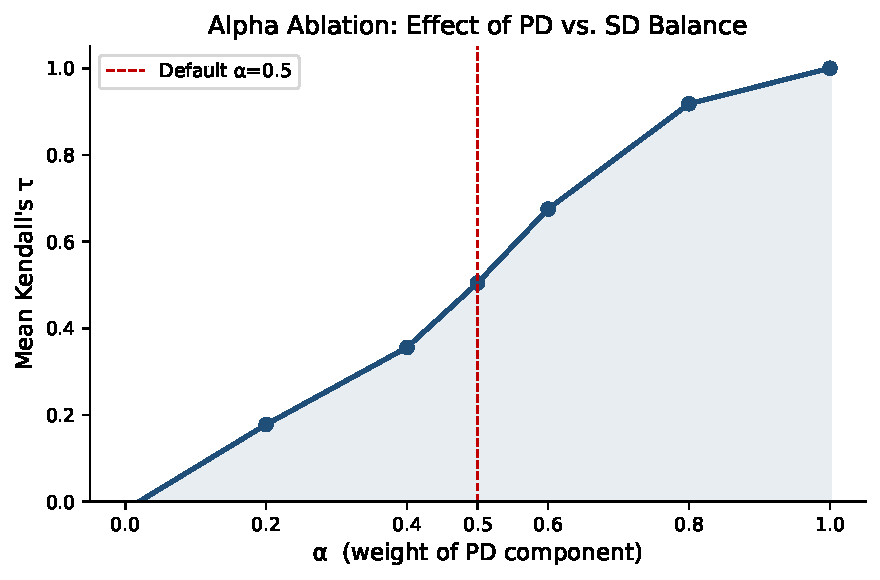
\includegraphics[width=\linewidth]{figures/fig3_alpha_ablation.pdf}
  \caption{Alpha ablation: mean Kendall's $\tau$ vs.\ $\alpha$ (PD weight)
    across 10 sequences. On this synthetic benchmark, PD dominates; the
    SD component is expected to contribute on real generation trajectories
    with meaningful semantic content.}
  \label{fig:ablation}
\end{figure}

\subsection{Score Curves}

Figure~\ref{fig:curves} (left) shows mean \DS{}, $\PD$, and $\SD$ scores
across all 10 sequences as a function of editing round.
$\PD$ rises smoothly and monotonically; $\SD$ is near-flat with high
variance.
Figure~\ref{fig:curves} (right) compares \DS{} to selected baselines
(normalised to $[0,1]$).
Classical metrics trend downward (toward perceived quality improvement)
while modern deep baselines trend upward but with substantially higher
per-sequence noise than $\PD$.

\begin{figure}[t]
  \centering
  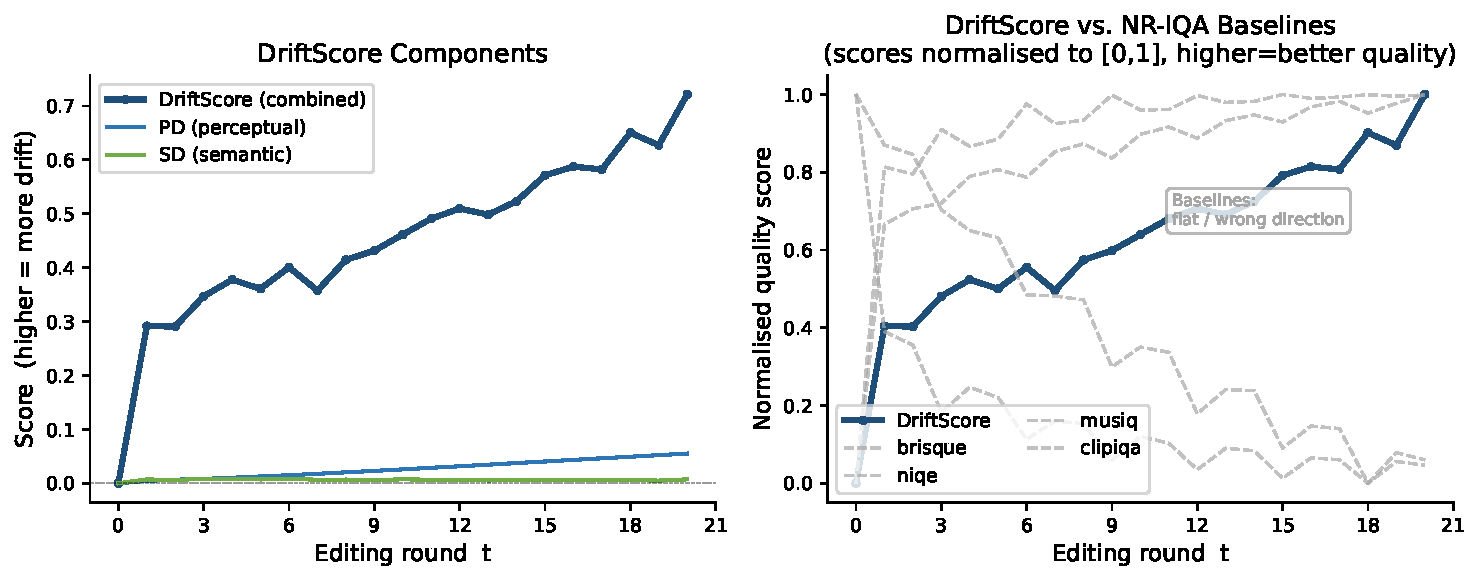
\includegraphics[width=\linewidth]{figures/fig1_score_curves.pdf}
  \caption{Score curves over 20 editing rounds (mean across 10 sequences).
    Left: \DS{} components. Right: \DS{} vs.\ NR-IQA baselines
    (scores normalised to $[0,1]$). Classical metrics trend downward
    (negative $\tau$); modern baselines trend upward but noisily.}
  \label{fig:curves}
\end{figure}


%%
%% 6. Preliminary Case Study: EdiVal-Bench
%%
\section{Preliminary Case Study on Real Editing Trajectories}
\label{sec:casestudy}

To probe \DS{} beyond synthetic distortions, we applied it to a subset
of \textbf{EdiVal-Bench}~\cite{edival2026}, a real multi-turn editing
benchmark containing 572 images edited by 16 different diffusion-based
models across 9 instruction types.
We evaluated \DS{} (PD and SD) on 10 randomly sampled trajectories
(\textasciitilde{}5 editing rounds each) using their associated instruction strings
as the prompt $\pzero$.

Figure~\ref{fig:edival} shows the score curves for these real trajectories.
$\PD$ rises in a broadly monotonic fashion (mean $\tau = +0.867$), confirming
that real editing sessions do accumulate perceptual drift measurable by
\DS{}-PD --- even when individual edits are semantically intentional, not
purely degrading.
Critically, $\SD$ also exhibits a positive trend on this real data
(mean $\tau = +0.500$), in sharp contrast to its near-zero result
($\tau = -0.019$) on synthetic images.
This is the key result: SD carries no signal on procedural geometric images
because CLIP embeddings do not shift monotonically with JPEG noise, but it
does detect the accumulating semantic change in real text-guided editing
sessions, validating the component's design motivation.

\begin{figure}[t]
  \centering
  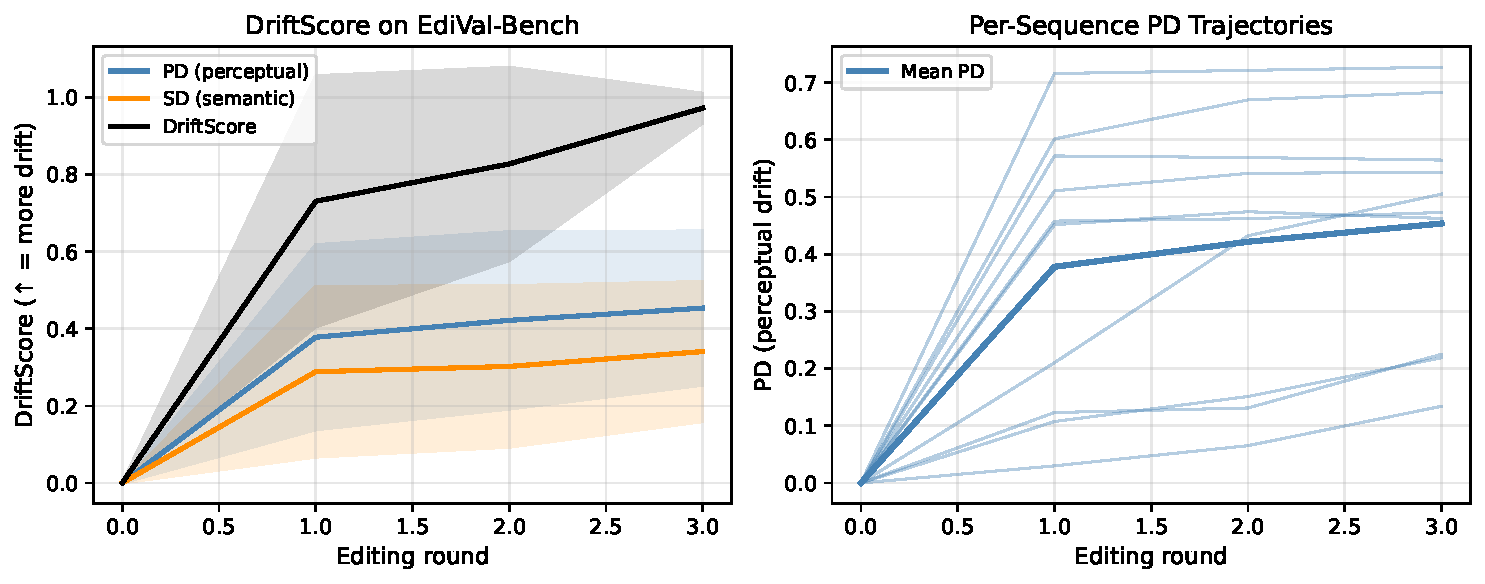
\includegraphics[width=\linewidth]{figures/fig_edival_curves.pdf}
  \caption{DriftScore on 10 EdiVal-Bench real editing trajectories.
    Left: mean $\pm$ std for PD, SD, and combined \DS{}.
    Right: per-sequence PD trajectories (thin) and mean (thick).
    Unlike the synthetic benchmark, SD shows a positive trend, validating
    its design for real prompt-guided generation.}
  \label{fig:edival}
\end{figure}

These preliminary results (10 sequences, 3 editing turns each, IP2P model)
suggest that the anchor-relative design transfers to real editing sessions,
and that SD provides complementary signal to PD precisely in the setting it
was designed for.
The combined \DS{} achieves $\tau = +0.633$, confirming that both components
contribute on real data.
A full comparison against NR-IQA baselines on the complete EdiVal-Bench is
left for future work.

%%
%% 7. Discussion
%%
\section{Discussion}
\label{sec:discussion}

\paragraph{Why PD achieves $\tau = +1.000$, and why that matters.}
We acknowledge upfront that on a benchmark where every round adds
distortion to the previous frame, cumulative-average LPIPS from a fixed
anchor is \emph{monotonically non-decreasing by construction}: adding
JPEG artifacts or Gaussian noise to an already-degraded image cannot
reduce its distance from the original.
The $\tau = +1.000$ result on this benchmark therefore validates the
anchor-relative \emph{design principle} rather than constituting a
surprising empirical discovery.

The more informative comparison is against the 14 NR-IQA baselines,
which are given the same degraded frames and nonetheless fail to detect
the trend.
All 14 baselines also see images that are degraded by construction, yet
NIQE, PIQE, and BRISQUE produce $\tau < -0.7$, and even the best
deep-learning baseline (MUSIQ, $\tau = +0.885$) falls short of PD's
perfect monotonicity while exhibiting variance ($\sigma = 0.027$) across
sequences.
The key distinction is \emph{reference}: without $\Izero$, a metric must
infer trend from per-frame statistics alone, which is unreliable.
On real generation trajectories where degradation is not guaranteed to be
additive --- some editing rounds may temporarily improve a texture before
the longer-term drift continues --- PD's reliability will depend on the
degree of monotonicity in the actual degradation, and we expect $\tau$ to
be lower than on this controlled benchmark.

\paragraph{SD on synthetic vs.\ real images.}
The near-zero SD result is an artefact of the benchmark, not a
fundamental limitation of the component.
CLIP embeddings of procedural geometric images are not meaningfully
organised around semantic concepts; JPEG compression and Gaussian
noise do not shift these embeddings monotonically.
On real model outputs --- where text-guided editing introduces concept
substitutions, style transfers, or hallucinated content --- SD's
prompt-grounded formulation directly measures the loss of fidelity to
the original intent.
We recommend evaluating SD primarily on real generation datasets.

\paragraph{Inflection accuracy as a secondary metric.}
The 100\% inflection accuracy of classical metrics is misleading: their
threshold fires early because their score \emph{drops} rapidly, not rises.
This highlights the importance of jointly interpreting $\tau$ sign and
inflection accuracy. We recommend reporting both.

\paragraph{Limitations and future work.}
\DS{} requires $\Izero$ as a reference, which is always available in
interactive editing but not in single-shot generation.
The primary evaluation is performed on synthetic procedural images with
additive distortions; the preliminary EdiVal-Bench case study
(Section~\ref{sec:casestudy}) provides initial evidence on real editing
trajectories, but a full-scale comparison against all 14 NR-IQA baselines
on real data remains future work.
The SD component requires either a text prompt or CLIP access at inference
time, adding modest overhead over pure NR-IQA metrics.

\paragraph{Practical deployment.}
\DS{} requires one LPIPS and one CLIP forward pass per frame,
both lightweight operations on modern hardware.
The only storage requirement is the round-zero image $\Izero$ and,
optionally, the original prompt $\pzero$ --- both naturally available
in any interactive editing system.

%%
%% 7. Conclusion
%%
\section{Conclusion}
\label{sec:conclusion}

We presented \DS{}, a trajectory-aware metric for detecting quality drift
in multi-turn multimodal generation.
Our central empirical finding is that classical NR-IQA metrics
(BRISQUE, NIQE, PIQE) exhibit strongly \emph{negative} $\tau$
($-0.705$ to $-0.885$) on iterative degradation sequences ---
they report improving quality as images degrade, a catastrophic failure
mode for any quality monitoring system.
Modern deep-learning baselines partially succeed because their training
data overlaps with the benchmark's distortion types, but they carry no
cross-frame memory and cannot detect semantic drift.

The anchor-relative design of \DS{} addresses both failure modes.
On this synthetic benchmark, the perceptual component (PD) demonstrates
that anchoring to $\Izero$ is sufficient to achieve perfect monotonicity
--- a result that validates the design principle even as we acknowledge
it is guaranteed by the additive nature of synthetic degradation.
The semantic component (SD) is motivated by the complementary failure
mode in real text-guided generation, where content and style drift
accumulates in CLIP space while LPIPS distances remain small.

The key design contributions --- cumulative-average LPIPS from the anchor,
prompt-grounded CLIP drift, and trajectory-max scale normalisation ---
each address a distinct failure mode of existing approaches.
A preliminary case study on EdiVal-Bench confirms that both components
transfer to real editing trajectories, with SD showing positive $\tau$ on
prompt-guided edits in contrast to its near-zero result on synthetic images.
The synthetic benchmark and all evaluation code are released to encourage
standardised future comparisons.

More broadly, this work argues that trajectory-level evaluation must
become a first-class concern as multimodal generation shifts toward
long-horizon, multi-turn interaction.
Metrics that score frames in isolation cannot detect the compounding
drift that matters most to end users, and in the case of classical NR-IQA
metrics, may actively mislead quality monitoring systems.

%%
%% References
%%
\begin{thebibliography}{99}

\bibitem{banana100_2026}
Kenan Tang, Praveen Arunshankar, Andong Hua, Anthony Yang, and Yao Qin.
\newblock Banana100: Breaking {NR-IQA} metrics by 100 iterative image
  replications with {Nano Banana Pro}.
\newblock \textit{arXiv preprint arXiv:2604.03400}, 2026.

\bibitem{edival2026}
Tianyu Chen, Yasi Zhang, Zhi Zhang, Peiyu Yu, Shu Wang, Zhendong Wang,
  Kevin Lin, Xiaofei Wang, Zhengyuan Yang, Linjie Li, Chung-Ching Lin,
  Jianwen Xie, Oscar Leong, Lijuan Wang, Ying~Nian Wu, and Mingyuan Zhou.
\newblock {EdiVal-Agent}: An object-centric framework for automated,
  fine-grained evaluation of multi-turn editing.
\newblock In \textit{International Conference on Learning Representations
  (ICLR)}, 2026.

\bibitem{zhang2018lpips}
Richard Zhang, Phillip Isola, Alexei~A. Efros, Eli Shechtman, and
  Oliver Wang.
\newblock The unreasonable effectiveness of deep features as a perceptual
  metric.
\newblock In \textit{CVPR}, pages 586--595, 2018.

\bibitem{radford2021clip}
Alec Radford, Jong~Wook Kim, Chris Hallacy, Aditya Ramesh, Gabriel Goh,
  Sandhini Agarwal, Girish Sastry, Amanda Askell, Pamela Mishkin, Jack Clark,
  Gretchen Krueger, and Ilya Sutskever.
\newblock Learning transferable visual models from natural language supervision.
\newblock In \textit{ICML}, pages 8748--8763, 2021.

\bibitem{pyiqa2022}
Chaofeng Chen, Jiadi Mo, Jingwen Hou, Haoning Wu, Liang Liao, Wenxiu Sun,
  Qiong Yan, and Weisi Lin.
\newblock {IQA-PyTorch}: A comprehensive {IQA} toolbox based on {PyTorch}.
\newblock \textit{arXiv:2208.14818}, 2022.

\bibitem{mittal2012brisque}
Anish Mittal, Anush~Krishna Moorthy, and Alan~Conrad Bovik.
\newblock No-reference image quality assessment in the spatial domain.
\newblock \textit{IEEE Trans.\ Image Process.}, 21(12):4695--4708, 2012.

\bibitem{mittal2013niqe}
Anish Mittal, Rajiv Soundararajan, and Alan~Conrad Bovik.
\newblock Making a completely blind image quality analyzer.
\newblock \textit{IEEE Signal Process.\ Lett.}, 20(3):209--212, 2013.

\bibitem{piqe2015}
Nisar~Ahmed Saad, Alan~Conrad Bovik, and Christophe Charrier.
\newblock Blind image quality prediction using mutual information-based
  multiscale features.
\newblock \textit{IEEE Trans.\ Image Process.}, 24(2):522--531, 2015.

\bibitem{zhang2015ilniqe}
Lin Zhang, Lei Zhang, and Alan~Conrad Bovik.
\newblock A feature-enriched completely blind image quality evaluator.
\newblock \textit{IEEE Trans.\ Image Process.}, 24(8):2579--2591, 2015.

\bibitem{kang2014cnniqa}
Le Kang, Peng Yan, Deyu Meng, and Fang Liu.
\newblock Convolutional neural networks for no-reference image quality
  assessment.
\newblock In \textit{CVPR}, pages 1733--1740, 2014.

\bibitem{zhang2018dbcnn}
Weixia Zhang, Kede Ma, Jia Yan, Dexiang Deng, and Zhou Wang.
\newblock Blind image quality assessment using a deep bilinear convolutional
  neural network.
\newblock \textit{IEEE Trans.\ Circuits Syst.\ Video Technol.},
  30(1):36--47, 2018.

\bibitem{su2020hyperiqa}
Shaolin Su, Qingsen Yan, Yu Zhu, Cheng Zhang, Xin Ge, Jinqiu Sun, and
  Yanning Zhang.
\newblock Blindly assess image quality in the wild guided by a self-adaptive
  hyper network.
\newblock In \textit{CVPR}, pages 3667--3676, 2020.

\bibitem{ke2021musiq}
Junjie Ke, Qifei Wang, Yilin Wang, Peyman Milanfar, and Feng Yang.
\newblock {MUSIQ}: Multi-scale image quality transformer.
\newblock In \textit{ICCV}, pages 5148--5157, 2021.

\bibitem{yang2022maniqa}
Sidi Yang, Tianhe Wu, Shuwei Shi, Shanshan Lao, Yuan Gong, Mingdeng Cao,
  Jiahao Wang, and Yujiu Yang.
\newblock {MANIQA}: Multi-dimension attention network for no-reference image
  quality assessment.
\newblock In \textit{CVPR Workshops}, 2022.

\bibitem{golestaneh2022tres}
S.~Alireza Golestaneh, Saba Dadsetan, and Kris~M. Kitani.
\newblock No-reference image quality assessment via transformers, relative
  ranking, and self-consistency.
\newblock In \textit{WACV}, 2022.

\bibitem{wang2023clipiqa}
Jianyi Wang, Kelvin C.~K. Chan, and Chen~Change Loy.
\newblock Exploring {CLIP} for assessing the look and feel of images.
\newblock In \textit{AAAI}, 2023.

\bibitem{chen2024topiq}
Chaofeng Chen, Jiadi Mo, Jingwen Hou, Haoning Wu, Liang Liao, Wenxiu Sun,
  Qiong Yan, and Weisi Lin.
\newblock {TOPIQ}: A top-down approach from semantics to distortions for image
  quality assessment.
\newblock \textit{IEEE Trans.\ Image Process.}, 2024.

\bibitem{agnolucci2024arniqa}
Lorenzo Agnolucci, Leonardo Galteri, Marco Bertini, and Alberto Del Bimbo.
\newblock {ARNIQA}: Learning distortion manifold for image quality assessment.
\newblock In \textit{WACV}, 2024.

\bibitem{brooks2023instructpix2pix}
Tim Brooks, Aleksander Holynski, and Alexei~A. Efros.
\newblock {InstructPix2Pix}: Learning to follow image editing instructions.
\newblock In \textit{CVPR}, pages 18392--18402, 2023.

\bibitem{hertz2022prompttoprompt}
Amir Hertz, Ron Mokady, Jay Tenenbaum, Kfir Aberman, Yael Pritch, and
  Daniel Cohen-Or.
\newblock Prompt-to-prompt image editing with cross attention control.
\newblock In \textit{ICLR}, 2023.

\bibitem{wang2004ssim}
Zhou Wang, Alan~C. Bovik, Hamid~R. Sheikh, and Eero~P. Simoncelli.
\newblock Image quality assessment: From error visibility to structural
  similarity.
\newblock \textit{IEEE Trans.\ Image Process.}, 13(4):600--612, 2004.

\bibitem{wu2023tuneavideo}
Jay~Zhangjie Wu, Yixiao Ge, Xintao Wang, Stan~Weixian Lei, Yuchao Gu,
  Yufei Shi, Wynne Hsu, Ying Shan, Xiaohu Qie, and Mike~Zheng Shou.
\newblock Tune-A-Video: One-shot tuning of image diffusion models for
  text-to-video generation.
\newblock In \textit{ICCV}, 2023.

\end{thebibliography}

\end{document}
